\documentclass{acaces}

\usepackage{wrapfig}

\begin{document}

\title{"\textit{Smart}" Manual Software Parallelisation Assistant}

\author{
Aleksandr~Maramzin\addressnum{1}\extranum{1},
Bj\"{o}rn Franke\addressnum{1}\extranum{2},
Murray Cole\addressnum{1}\extranum{2}
}

\address{1}{
Institute For Computing Systems Architecture, 
Informatics Forum, 
The University of Edinburgh, 
10 Crichton Street, 
Edinburgh, 
UK
}

\extra{1}{E-mail: s1736883@sms.ed.ac.uk}
\extra{2}{E-mail: \{bfranke,mic\}@inf.ed.ac.uk}

\pagestyle{empty}

\begin{abstract}
\null\quad Since automatically parallelizing compilers have failed to deliver significant performance improvements, programmers are still forced to parallelize legacy software manually. Rather than hoping for an elegant silver bullet, we acknowledge the role of a human expert in the parallelization process and develop a \textit{smart} parallelization assistant.\newline\null
\quad In its essence our assistant is yet another application of machine learning (ML) techniques to the field of optimizing compilers, which tries to predict the parallelisability property of program loops. We use Seoul National University version of NAS Parallel Benchmarks (NPB) hand-annotated with OpenMP parallelisation pragmas to train our ML model. We show that  our problem can be successfully tackled with ML techniques achieveing the accuracy of around 90\% and outperforming all available baseline random predictors working at an accuracy ranging between 40\% and 70\%.\newline\null
\quad To get a real practical application of our techniques, we integrate our trained predictor into an assistant scheme, designed to mitigate the effects of ineradicable statistical errors. Taking application profile our assistant directs a programmer's efforts by pointing the loops, which are "highly likely" to be parallelisible and profitable as well. The latter eases and accelerates the manual parallelization process. 
\end{abstract}

\keywords{ACACES; poster session; software engineering; parallel programming; compilers; static program dependence analysis; loop iterator recognition; machine learning; programmer feedback;}

\section{Introduction}
\quad Automatically parallelizing compilers do not achieve the levels of performance expert programmers do. As our preliminary experiments show the effects that Intel C/C++ Compiler (ICC) had with its vectorizing and parallelizing transformations on SNU NPB benchmarks ranged from no change to a significant slowdown. Rarely ICC vectorization was able to achieve a tiny speedup, but the former faded in comparison with the speedup of an expertly parallelised SNU NPB OpenMP version. Hence, in our work we do not aim to replace a human expert, but provide the latter with an additional guidance on how to parallelise the program.\newline\null
\quad Our assistant is based on an ML model, trained to classify program loops as parallelisible or not. We use SNU NPB benchmarks hand-annotated with OpenMP parallelisation pragmas. The latter are used as loop classification labels. We supplement these labels with an additional information parsed out of ICC optimization reports.\newline\null
\quad The application of ML techniques to the field of optimizing compilers is not a new endeavour. There have been numerous successful attempts: selecting the best compiler flags, determining how to map parallelism to processors, etc. For these types of problems uneradicable statistical errors inherent to all ML techniques might result in the performance losses, but do not compromise the functional correctness. In our work we step into a potentially dangerous area. Loops wrongly predicted as parallel can break the program. There is an already published work \cite{fried_ea:2013:icmla} studying the possibility of learning loop parallleisability property. The answer is "yes" and the work reports on a predictive performance authors achieved. But the work does not step any further to actually find any practical applications. Moreover, the data set is highly unbalanced, which sets the baseline accuracy very high. Authors use dynamic program features.\newline\null
\quad On the contrary, we work with a more balanced data set, based on richer sources of information to derive classification labels from. At the end we harness our trained ML model into a practical application scheme.
\section{Predicting Parallel Loops}
\label{predicting_parallel_loops}
\begin{figure}
	\centering
	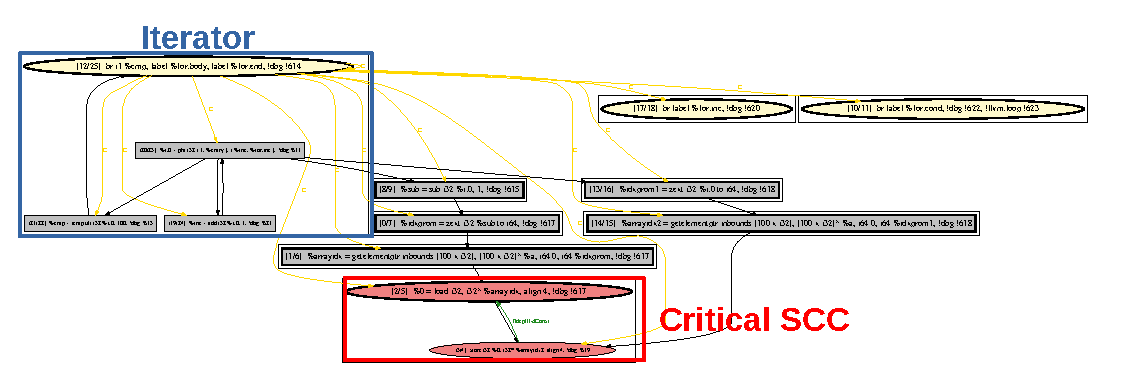
\includegraphics[width=1.0\textwidth]{pdg_example}
	\caption{Program Dependence Graph of a simple loop with recognised iterator, regular and critical payload parts. Nodes are LLVM IR instructions, edges are different types of dependencies between them.}
	\label{fig:pdg}
\end{figure}
\quad We pose a \textit{\textbf{supervised machine learning (ML) classification problem}}: create an ML based model and train it to classify loops of SNU NPB benchmarks as parallelizable or not. Our work encompasses two technical aspects. First, we need to find a representative set of quantifiable features, which would accurately reflect the parallelisability property of program loops, then we need to select the exact ML training/testing methodology to employ for our problem. Our features and the exact parameters of methodology (automatic feature selection methods, ML models and their hyper-parameter spaces, etc.) have been iteratively tuned with the help of K-fold CV. Predictive accuracy, recall and precision scores were used as the main selection criteria. We used facilities of \textbf{\textit{scikit-learn}} Python library for all ML related tasks.
\begin{wraptable}{h!}{0.5\textwidth}
	\centering
	\begin{tabular}[c]{|p{1.5cm}|p{1.5cm}|p{1.5cm}|p{1.5cm}|}
		\hline
		ML model & accuracy & recall & precision \\
		\hline
		constant & 70.32 & 100 & 70.32\\
		\hline
		uniform & 46.27 & 41.50 & 69.79\\
		\hline
		SVC & 90.04 & 95.24 & 91.06 \\
		\hline
		AdaBoost & 86.96 & 92.92 & 89.06 \\
		\hline
		DT & 84.36 & 89.57 & 87.90 \\
		\hline
		RFC & 86.65 & 93.22 & 88.47 \\
		\hline
		MLP & 89.40 & 93.77 & 91.39 \\
		\hline
	\end{tabular}
	\caption{Average predictive performance for different ML models measured with a K-fold CV method on the whole set of 1415 SNU NPB loops.}
	\label{tab:accuracy}
\end{wraptable}
\quad In the task of coming up with a set of loop features we are guided by the general program dependence analysis theory, insights into SNU NPB benchmarks and ICC optimization reports. There is a range of SNU NPB loops, which escape Intel compiler parallelisation for different reasons, but all of them are going to ultimately materialise into data and control dependencies present between loop instructions, represented as edges on the loop's Program Dependence Graph (PDG). To refine our features we conduct a generalised loop iterator recognition \cite{Manilov:2018:GPI:3178372.3179511} analysis on the PDG graph. Figure \ref{fig:pdg} shows an example of a PDG built for a simple loop and visualised with our tool. We base our loop features on a static structural properties of PDG. There are 74 different features we use, which are simplistic and defined as different numbers and fractions calculated on a graphs: numbers of particular LLVM IR instructions (calls, loads, stores, branches, etc.), numbers of various dependence edges (true, anti, output, etc.), sizes of iterators and payloads, etc.\newline\null
\begin{figure}
	\centering
	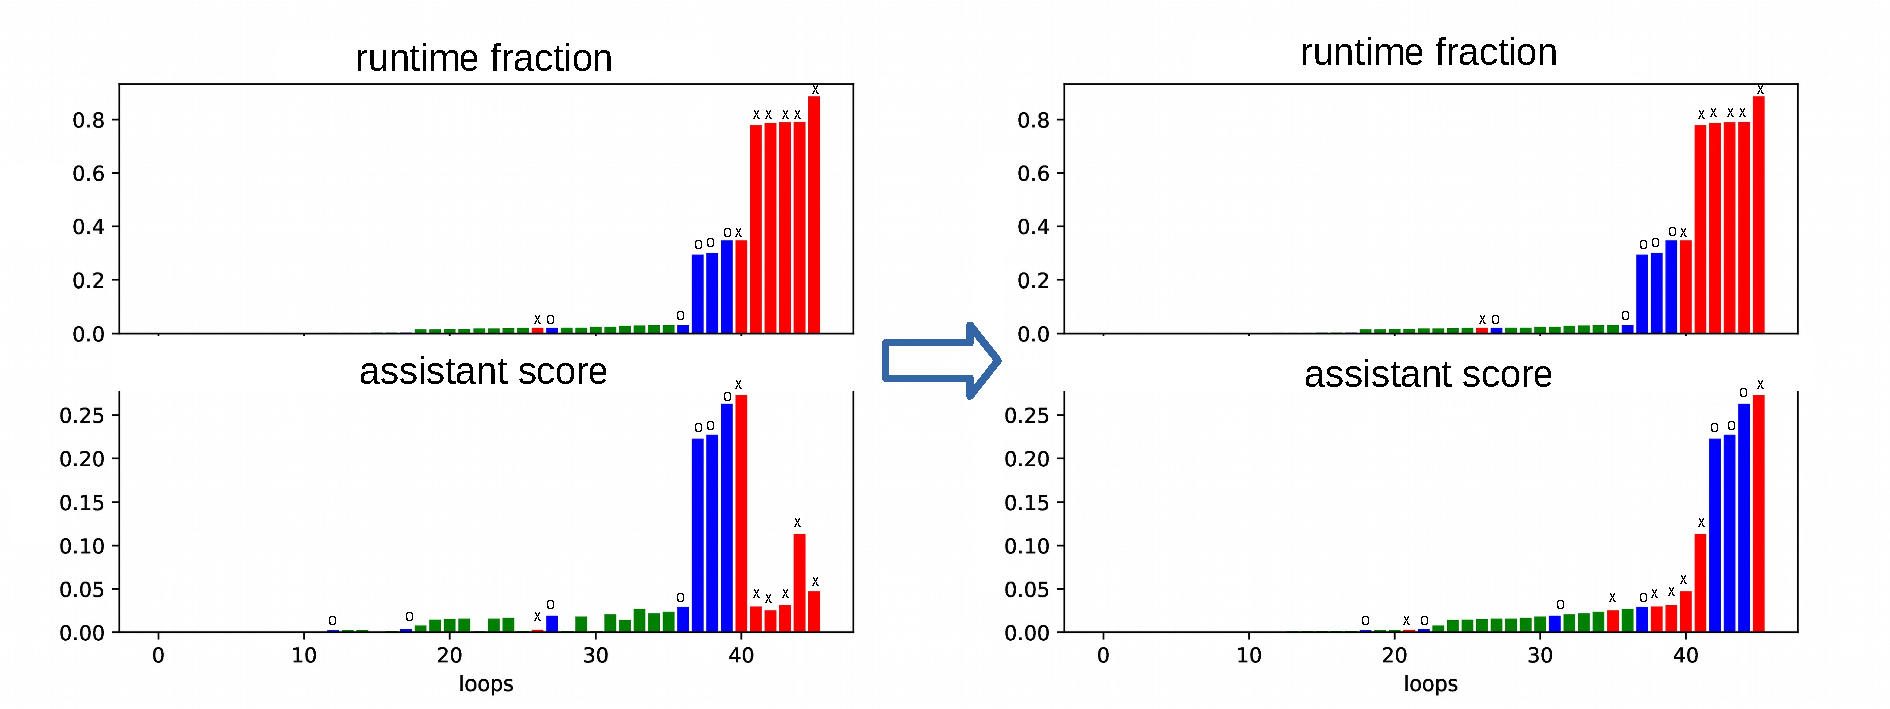
\includegraphics[width=1.0\textwidth]{ft_ranking}
	\caption{Illustration of loop ranking transformation. We multiply loop runtime on the shifted sigmoid function of loop parallelisability probability, thus amplifying parallel loops and extinguishing non-parallel ones. }
	\label{ranking}
\end{figure}
\quad The final predictive performance depends not only on the successful choice of features, but on the exact training and testing methodology as well. The latter is composed of a number of pipeline stages. We start with data preprocessing and automatic feature selection (low variance feature elimination, tree based methods, RFECV, etc.) in order to exclude redundant and irrelevant features, which lead to model over-fitting. Then we choose the exact ML model (SVC, DT, RFC, MLP, AdaBoost) to use and tune its hyper-parameters. And finally, we conduct the actual training and testing with standard K-fold and modified Leave-One-Out Cross-Validation (LOOCV)  techniques described in the literature. While K-fold method averages accuracy scores on different data set splits and can be used for feature selection, hyper-parameter tuning and overall predicitve performance estimation, modified LOOCV can be applied against any single SNU NPB benchmark in order to assess our assistant scheme. Table \ref{tab:accuracy} reports on the achieved accuracy.
\begin{wrapfigure}{R}{0.5\textwidth}
	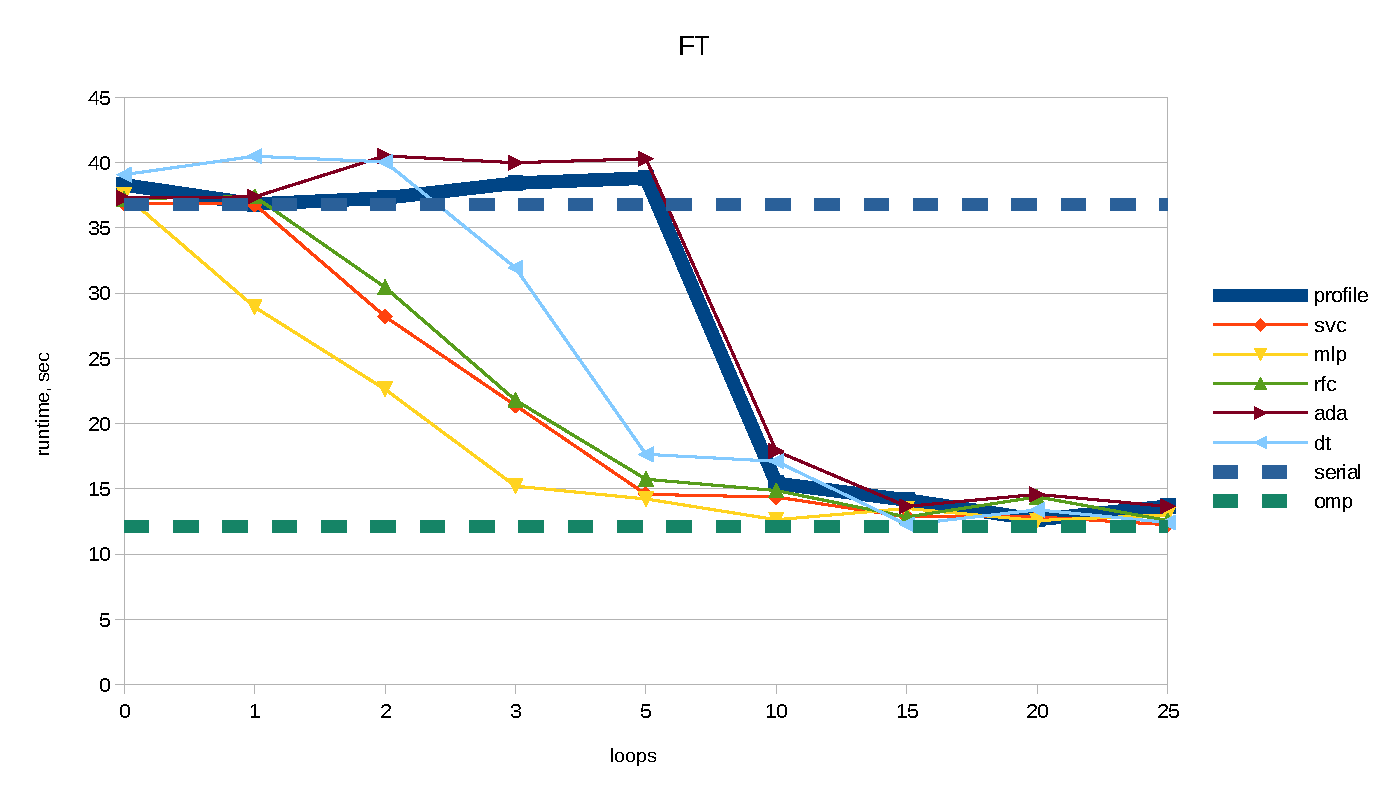
\includegraphics[width=0.5\textwidth]{ft_parallelisation}
	\caption{SNU NPB FT. Illustration of a faster convergence to the maximum achievable parallel software performance. Thick line is the profile loop order. Other lines represent improved rankings (instead of 10 loops we need only 3).}
	\label{convergence}
\end{wrapfigure}\null
\section{Manual Software Parallelization Assistant}
\label{predicting_parallel_loops}
\quad Achieving high prediction accuracy is not enough. We need to find a way to utilise our work practically. Since false positive mispredictions can break a program, we devised a scheme, which makes them less critical and leaves the question of final parallelisation up to a programmer to decide.\newline\null
\quad Our predictor is capable of discovering additional parallelisation opportunities, which escape the conservative analysis of ICC. For SNU NPB benchmarks we increse the amount of discovered parallelism from 81\% to 96\%. But not all parallel loops have to be parallelised. We are interested only in the loops, which take significant application runtime fraction and thus directly affect overall performance. Our assistant takes an application profile and reorders the list of loops, so that all long running non-parallel loops go to the back of the list. List's front highlights the loops to start parallelization with. Figure \ref{convergence} illustrates the principle. Parallelising the program by following the reorded list of loops, a programmer can get to the best achievable performance faster. Figure \ref{convergence} illustrates the process.   

\bibliography{guide}

\end{document}